\chapter{Resultados}
\label{chap:resultados}

Este capítulo apresenta e discute os resultados obtidos a partir dos experimentos descritos no Capítulo~\ref{chap:metodologia}. A análise busca verificar como as diferentes formas de recompensa e intensidades de glaucoma artificial influenciam o aprendizado, a sobrevivência e o comportamento dos agentes na tarefa \textit{Health-Gathering}. Para isso, são comparadas as condições sem recompensa, com recompensa extrínseca padrão e com recompensa intrínseca baseada em \textit{Random Network Distillation} (RND), conforme descrito na Seção~\ref{sec:configuracoes-experimentais}.

Conforme definido na Seção~\ref{sec:metricas-de-avaliacao}, os resultados são examinados por meio de dimensões complementares. Inicialmente, a duração média dos episódios é utilizada para comparar a evolução da capacidade de sobrevivência dos agentes ao longo do treinamento. Em seguida, as trajetórias produzidas diante de diferentes distribuições espaciais dos \textit{medikits} são analisadas para identificar se as políticas respondem à organização dos recursos ou apenas reproduzem padrões fixos de movimentação. Nas configurações baseadas em RND, também é investigada a relação entre recompensa intrínseca e precariedade perceptiva, com o objetivo de avaliar se a degradação da visão é efetivamente convertida em um sinal relevante para o aprendizado. Por fim, os mapas produzidos pelo Grad-CAM são examinados para identificar quais regiões das observações apresentam maior relevância para as decisões das políticas aprendidas. Essas análises permitem discutir não apenas o desempenho alcançado, mas também em que medida o mecanismo proposto favorece comportamentos relacionados à manutenção das condições de viabilidade do agente.

\section{Resultados por Força de Glaucoma}

Esta seção organiza os resultados de acordo com as configurações experimentais descritas na Seção~\ref{sec:configuracoes-experimentais} e com a força do glaucoma artificial aplicada ao agente. Serão analisadas, nesta ordem, as forças $50$, $100$, $200$ e $0$, permitindo observar como diferentes intensidades de degradação perceptiva afetam o aprendizado e o comportamento. Para manter um critério comum de comparação, cada condição será examinada a partir de quatro dimensões complementares. Serão consideradas a duração média dos episódios ao longo do treinamento, as trajetórias produzidas diante das diferentes distribuições de \textit{medikits}, a relação temporal entre recompensa intrínseca e precariedade nas execuções que utilizam RND e a análise visual das políticas por meio do Grad-CAM. Essa organização permite avaliar separadamente cada intensidade de glaucoma e, ao mesmo tempo, identificar padrões e diferenças entre as condições experimentais.

\subsection{Glaucoma de Força 50}

\subsubsection{Duração Média dos Episódios}

A Figura~\ref{fig:episode-length-50} apresenta a evolução da duração média dos episódios para as três condições de recompensa sob glaucoma de força $50$. As linhas representam as médias obtidas ao longo das diferentes sementes experimentais, enquanto as regiões sombreadas indicam a variabilidade entre as execuções. Como a duração máxima de um episódio é de $2100$ \textit{ticks}, valores próximos desse limite indicam que o agente conseguiu sobreviver durante praticamente todo o tempo disponível.

\begin{figure}[h!]
    \centering
    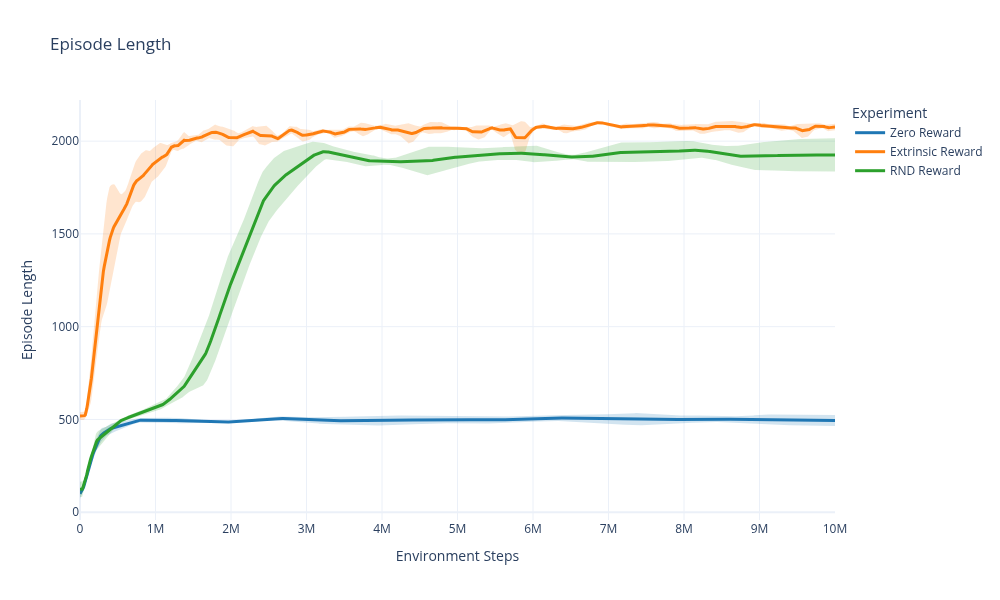
\includegraphics[width=0.9\linewidth]{figuras/episode_length_50.png}
    \caption{Duração média dos episódios ao longo do treinamento nas condições sem recompensa, com recompensa extrínseca e com recompensa intrínseca baseada em RND, sob glaucoma de força $50$. As regiões sombreadas representam a variabilidade entre as sementes experimentais.\\
    \textbf{Fonte:} Elaborada pelo autor.}
    \label{fig:episode-length-50}
\end{figure}

Na condição sem recompensa, a duração dos episódios cresce apenas nas etapas iniciais e se estabiliza em torno de $500$ \textit{ticks}. A ausência de crescimento posterior indica que o PPO, sem um sinal de reforço que diferencie as experiências, não aprende uma política capaz de prolongar sistematicamente a sobrevivência. Esse resultado é compatível com a função dessa condição como controle negativo do experimento.

Com a recompensa extrínseca, a duração aumenta rapidamente e se aproxima do limite máximo antes de $2$ milhões de passos. Depois desse período, o desempenho permanece estável em torno de $2000$ a $2100$ \textit{ticks}, com baixa variabilidade entre as sementes. Esse comportamento indica que o agente aprende a coletar \textit{medikits} e, como consequência, prolongar sua permanência no ambiente quando essas ações são diretamente valorizadas pelo projetista.

Na condição com recompensa intrínseca calculada pelo RND, o crescimento é mais lento. A duração permanece abaixo de $1000$ \textit{ticks} durante aproximadamente os primeiros $1{,}5$ milhão de passos e aumenta de forma acentuada entre $1{,}5$ e $3$ milhões de passos. Após esse período, estabiliza-se próxima de $1900$ \textit{ticks}, abaixo da recompensa extrínseca, mas muito acima da condição sem recompensa. A maior dispersão observada durante a fase de crescimento indica que a velocidade de aprendizado varia entre as sementes. Ainda assim, a convergência para episódios longos mostra que a recompensa intrínseca associada à precariedade foi suficiente para favorecer uma política sem recompensar diretamente a coleta de \textit{medikits}.

\subsubsection{Análise das Trajetórias}

A Figura~\ref{fig:trajectories-50} apresenta as trajetórias dos agentes nas distribuições em quadrado, círculo, seno e \textit{grid}. As trajetórias foram obtidas em episódios de avaliação executados com as políticas salvas após $9\,633\,792$ passos de treinamento. Esse checkpoint corresponde a um estágio avançado e próximo do orçamento total de $10$ milhões de passos, no qual as curvas de duração dos episódios já se encontravam estabilizadas. Sua utilização permite examinar o comportamento desenvolvido pelas políticas após uma quantidade ampla de experiências. As colunas correspondem às condições sem recompensa, com recompensa extrínseca e com recompensa intrínseca calculada pelo RND. A comparação permite verificar se as políticas respondem à organização espacial dos recursos ou apenas reproduzem uma forma geral de deslocamento.

\begin{figure}[h!]
    \centering
    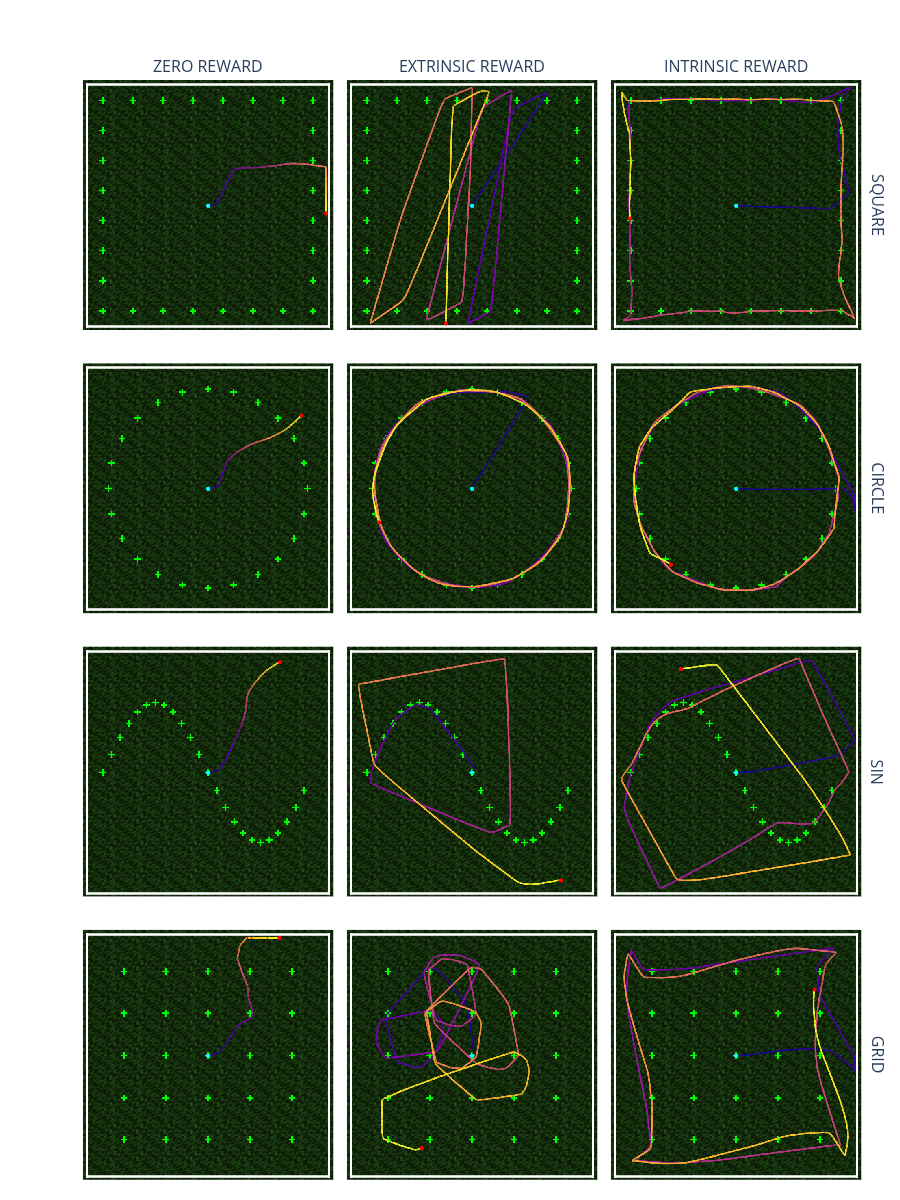
\includegraphics[width=1.0\linewidth]{figuras/trajectory_grid_50.png}
    \caption{Trajetórias produzidas pelas políticas salvas após $9\,633\,792$ passos de treinamento nas distribuições em quadrado, círculo, seno e \textit{grid}, sob as condições sem recompensa, com recompensa extrínseca e com recompensa intrínseca baseada em RND, para glaucoma de força $50$.\\
    \textbf{Fonte:} Elaborada pelo autor.}
    \label{fig:trajectories-50}
\end{figure}

Os agentes treinados sem recompensa percorrem trajetórias curtas e semelhantes nas quatro distribuições, afastando-se da posição inicial sem acompanhar a disposição dos \textit{medikits}. Esse comportamento reforça o resultado da duração dos episódios e não apresenta evidências de uma política orientada pela localização dos recursos.

Os agentes treinados com recompensa extrínseca exibem deslocamentos mais extensos, mas a correspondência com as distribuições varia entre os arranjos. Na configuração circular, as trajetórias acompanham claramente o círculo formado pelos recursos. Nas distribuições em quadrado, seno e \textit{grid}, porém, aparecem percursos amplos que atravessam regiões sem \textit{medikits} ou se concentram em apenas parte do ambiente. Mesmo sem reproduzir precisamente a geometria das distribuições, o agente consegue interceptar e coletar recursos, como indica a elevada duração dos episódios, prolongando sua permanência no ambiente. Uma possível explicação para os percursos mais amplos é a perda progressiva de visão causada pelo glaucoma. Com a observação parcialmente obstruída, o agente pode deixar de perceber \textit{medikits} próximos e continuar se deslocando até encontrar recursos ainda visíveis ou cruzá-los durante sua trajetória.

Na condição com recompensa intrínseca, as trajetórias acompanham de maneira clara os contornos das distribuições em quadrado, círculo e \textit{grid}. Na distribuição em seno, os percursos são mais dispersos e atravessam regiões externas à curva formada pelos \textit{medikits}. Esses resultados indicam que a política treinada com recompensas calculadas pelo RND utiliza informações espaciais do ambiente em parte das configurações e não se limita a repetir um único padrão de movimento.

\subsubsection{Relação entre Recompensa Intrínseca e Precariedade}

A Figura~\ref{fig:intrinsic-reward-50} apresenta a evolução conjunta da recompensa intrínseca e da precariedade perceptiva durante um episódio. As recompensas intrínsecas apresentadas foram calculadas pelo módulo RND após $200\,704$ passos de treinamento. Esse checkpoint, situado nas etapas iniciais do treinamento, foi utilizado porque o agente ainda não havia desenvolvido uma política altamente eficiente de coleta. Consequentemente, o episódio contém um intervalo prolongado sem contato com \textit{medikits}, durante o qual é possível observar o crescimento da precariedade e a redução da recompensa intrínseca. A coleta posterior permite examinar, no mesmo episódio, a restauração da visão e a resposta imediata do RND. Em estágios mais avançados, a coleta frequente dos recursos reduziria os intervalos de degradação contínua e dificultaria a visualização desse contraste. A linha tracejada representa o avanço do glaucoma, enquanto a estrela indica o instante em que um \textit{medikit} é coletado e a visão do agente é restaurada.

\begin{figure}[h!]
    \centering
    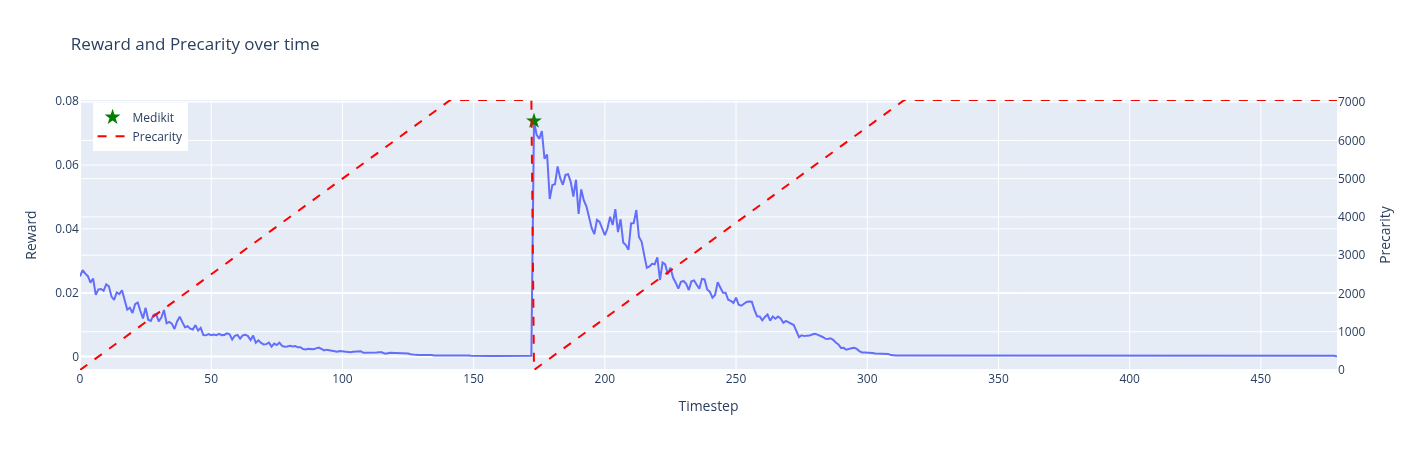
\includegraphics[width=0.9\linewidth]{figuras/intrinsic_reward_50.png}
    \caption{Evolução da recompensa intrínseca calculada pelo módulo RND após $200\,704$ passos de treinamento e da precariedade perceptiva ao longo de um episódio com glaucoma de força $50$. A estrela indica a coleta de um \textit{medikit} e a consequente restauração da visão.\\
    \textbf{Fonte:} Elaborada pelo autor.}
    \label{fig:intrinsic-reward-50}
\end{figure}

No início do episódio, a precariedade cresce continuamente, enquanto a recompensa intrínseca diminui até atingir valores próximos de zero. Quando a visão se encontra amplamente comprometida, a recompensa permanece praticamente nula. Esse comportamento indica que as observações degradadas se tornam previsíveis para a rede preditora do RND e deixam de produzir um sinal significativo de novidade.

Após a coleta do \textit{medikit}, aproximadamente no instante $170$, a precariedade retorna ao valor mínimo e a recompensa intrínseca apresenta seu maior pico no episódio. À medida que o glaucoma volta a crescer, a recompensa diminui novamente, aproximando-se de zero quando a precariedade alcança seu nível máximo. A repetição desse padrão antes e depois da coleta evidencia uma relação inversa entre as duas variáveis.

O resultado constitui um indício direto do mecanismo proposto nesta dissertação. A coleta do recurso não recebe uma recompensa programada, mas restaura uma condição perceptiva que produz maior erro de predição e, consequentemente, maior recompensa intrínseca. Assim, a condição menos precária adquire maior valor para o aprendizado por meio de seus efeitos sobre a percepção. Embora esse gráfico isolado não seja suficiente para estabelecer uma relação causal geral, sua dinâmica é consistente com a hipótese de conversão da precariedade corporal em recompensa.

\subsubsection{Análise Visual com Grad-CAM}

A Figura~\ref{fig:gradcam-50} apresenta mapas de Grad-CAM, método discutido na Seção~\ref{subsubsec:gradcam}, para as três condições de recompensa sob glaucoma de força $50$. A linha superior corresponde às políticas após $100\,352$ passos e a inferior às políticas após $9\,633\,792$ passos. As cores mais quentes indicam regiões com maior contribuição para a saída analisada da política, enquanto as mais frias indicam menor contribuição.

\begin{figure}[h!]
    \centering
    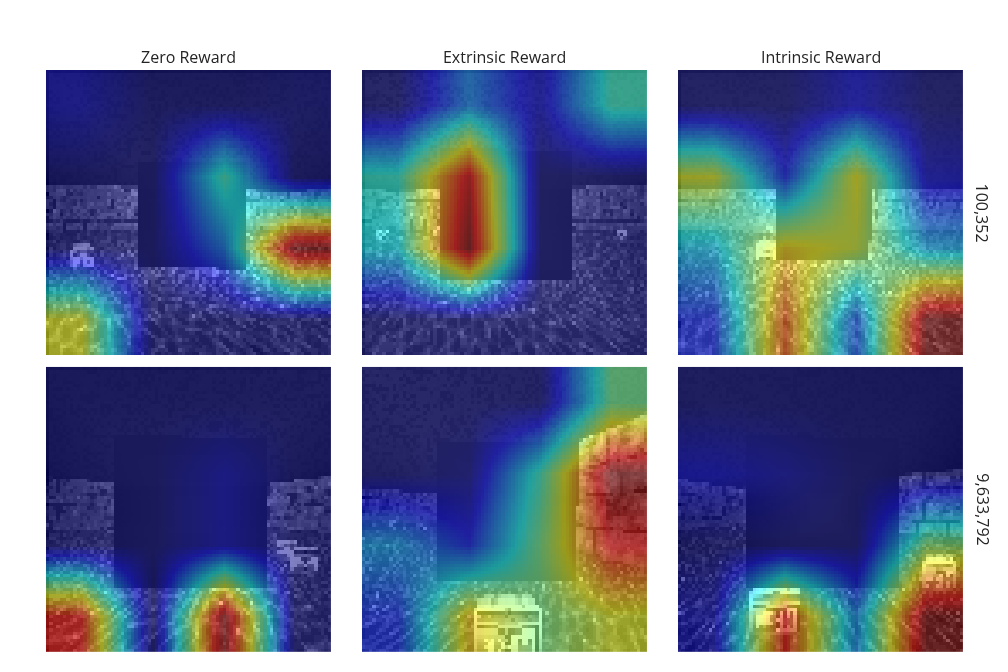
\includegraphics[width=1.0\linewidth]{figuras/gradcam_50.png}
    \caption{Mapas de Grad-CAM para as condições sem recompensa, com recompensa extrínseca e com recompensa intrínseca calculada pelo RND, sob glaucoma de força $50$. A linha superior apresenta as políticas após $100\,352$ passos de treinamento, e a linha inferior apresenta as políticas após $9\,633\,792$ passos. As regiões mais quentes possuem maior relevância para a saída analisada da política segundo o Grad-CAM.\\
    \textbf{Fonte:} Elaborada pelo autor.}
    \label{fig:gradcam-50}
\end{figure}

Na condição sem recompensa, os mapas inicial e final concentram as ativações nas porções inferiores da imagem e nas transições entre chão e paredes. O \textit{medikit} à esquerda no estágio inicial e o recurso na parede direita no estágio final não coincidem com as regiões de maior intensidade. Esse padrão, possivelmente relacionado a características visuais de baixo nível, como limites entre superfícies, texturas do chão e áreas próximas ao campo de deslocamento, é compatível com a ausência de evidências de que a política utilize os recursos para prolongar a sobrevivência.

Na condição com recompensa extrínseca, o mapa inicial se concentra em uma região vertical nas bordas da área escurecida pelo glaucoma, sem indicar direcionamento claro para os \textit{medikits} e aparentemente respondendo ao contraste nos limites da degradação visual. No estágio final, há relevância tanto sobre o recurso na região inferior quanto sobre a parede direita. A parede pode ser importante para evitar que o agente caminhe contra uma superfície ou mantenha a visão direcionada apenas para ela, deixando de observar o restante do ambiente. A política parece, portanto, combinar informações sobre recursos e geometria da sala, o que é coerente com trajetórias que permitem coletar itens e sobreviver sem reproduzir precisamente todas as distribuições.

Na condição com recompensa intrínseca, o mapa inicial é difuso, sem uma região dominante, e distribui relevância pelo corredor central, pelo chão e pela extremidade direita. No estágio final, as ativações tornam-se mais localizadas sobre elementos da parte inferior, incluindo um \textit{medikit} próximo ao centro e um objeto visualmente saliente à direita. Essa mudança é compatível com uma política que passou a diferenciar elementos potencialmente relevantes.

A comparação sugere usos distintos das informações visuais. A condição sem recompensa permanece associada a regiões genéricas do cenário, a recompensa extrínseca combina elementos de navegação e áreas próximas aos recursos, e a condição intrínseca passa a concentrar-se em objetos da região imediatamente navegável. Esse padrão constitui evidência qualitativa de que a política com recompensa intrínseca não responde apenas à degradação global, mas também utiliza estruturas espaciais e objetos da observação.

\subsection{Glaucoma de Força 100}

\subsubsection{Duração Média dos Episódios}

A Figura~\ref{fig:episode-length-100} apresenta a evolução da duração média dos episódios para as três condições de recompensa sob glaucoma de força $100$. Assim como na análise anterior, as linhas representam as médias entre as sementes experimentais e as regiões sombreadas mostram a dispersão correspondente a um desvio padrão.

\begin{figure}[h!]
    \centering
    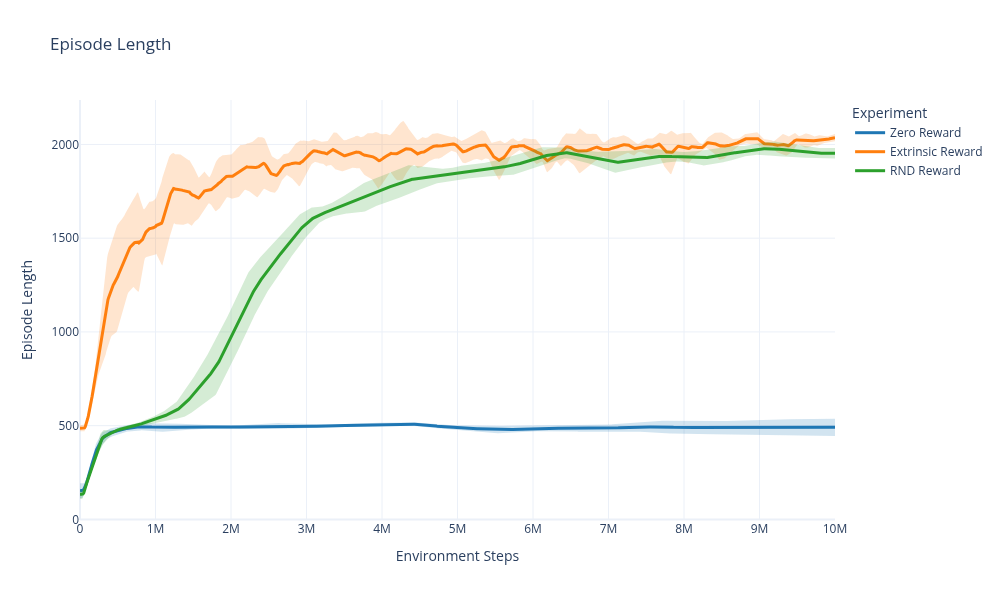
\includegraphics[width=0.9\linewidth]{figuras/episode_length_100.png}
    \caption{Duração média dos episódios ao longo do treinamento nas condições sem recompensa, com recompensa extrínseca e com recompensa intrínseca calculada pelo RND, sob glaucoma de força $100$. As regiões sombreadas representam a variabilidade entre as sementes experimentais.\\
    \textbf{Fonte:} Elaborada pelo autor.}
    \label{fig:episode-length-100}
\end{figure}

Na condição sem recompensa, a duração dos episódios se mantém próxima de $500$ \textit{ticks} durante praticamente todo o treinamento. A pequena variação observada não se transforma em uma tendência sustentada de crescimento, indicando novamente que a ausência de um sinal de reforço não permite ao agente aprender uma política capaz de coletar recursos e prolongar sua permanência no ambiente.

Com a recompensa extrínseca, a duração cresce rapidamente durante o primeiro milhão de passos, ultrapassando $1500$ \textit{ticks}. O crescimento continua de forma mais gradual até aproximadamente $3$ milhões de passos, quando a curva se aproxima de $1900$ a $2000$ \textit{ticks}. A variabilidade entre as sementes é elevada nas etapas iniciais, mas diminui à medida que as execuções convergem para episódios próximos da duração máxima. Esse resultado indica que, mesmo com a degradação mais rápida produzida pela força $100$, os agentes aprendem a coletar \textit{medikits} quando essa ação é diretamente recompensada.

Na condição com recompensa intrínseca calculada pelo RND, a duração permanece próxima de $500$ \textit{ticks} durante aproximadamente o primeiro milhão de passos. Entre $1$ e $3$ milhões de passos, observa-se um crescimento acentuado, acompanhado por uma faixa de desvio padrão mais ampla, o que indica diferenças na velocidade de aprendizado entre as sementes. Após esse período, a duração continua aumentando gradualmente e se aproxima da condição extrínseca entre $6$ e $7$ milhões de passos. Ao final do treinamento, ambas alcançam valores próximos de $2000$ \textit{ticks}. Portanto, embora o aprendizado orientado pela recompensa intrínseca seja mais lento, seus resultados finais mostram que o agente consegue desenvolver uma política de sobrevivência sem receber recompensa direta pela coleta de recursos.

\subsubsection{Análise das Trajetórias}

A Figura~\ref{fig:trajectories-100} apresenta as trajetórias obtidas nas quatro distribuições de \textit{medikits}. Os episódios de avaliação foram executados com as políticas salvas após $9\,533\,440$ passos de treinamento. Esse checkpoint está próximo do orçamento total de $10$ milhões de passos e corresponde a uma etapa na qual o desempenho das condições extrínseca e intrínseca já havia alcançado valores elevados e relativamente estáveis. Dessa forma, as trajetórias permitem examinar políticas em estágio avançado de treinamento, reduzindo a influência de comportamentos transitórios das etapas iniciais.

\begin{figure}[h!]
    \centering
    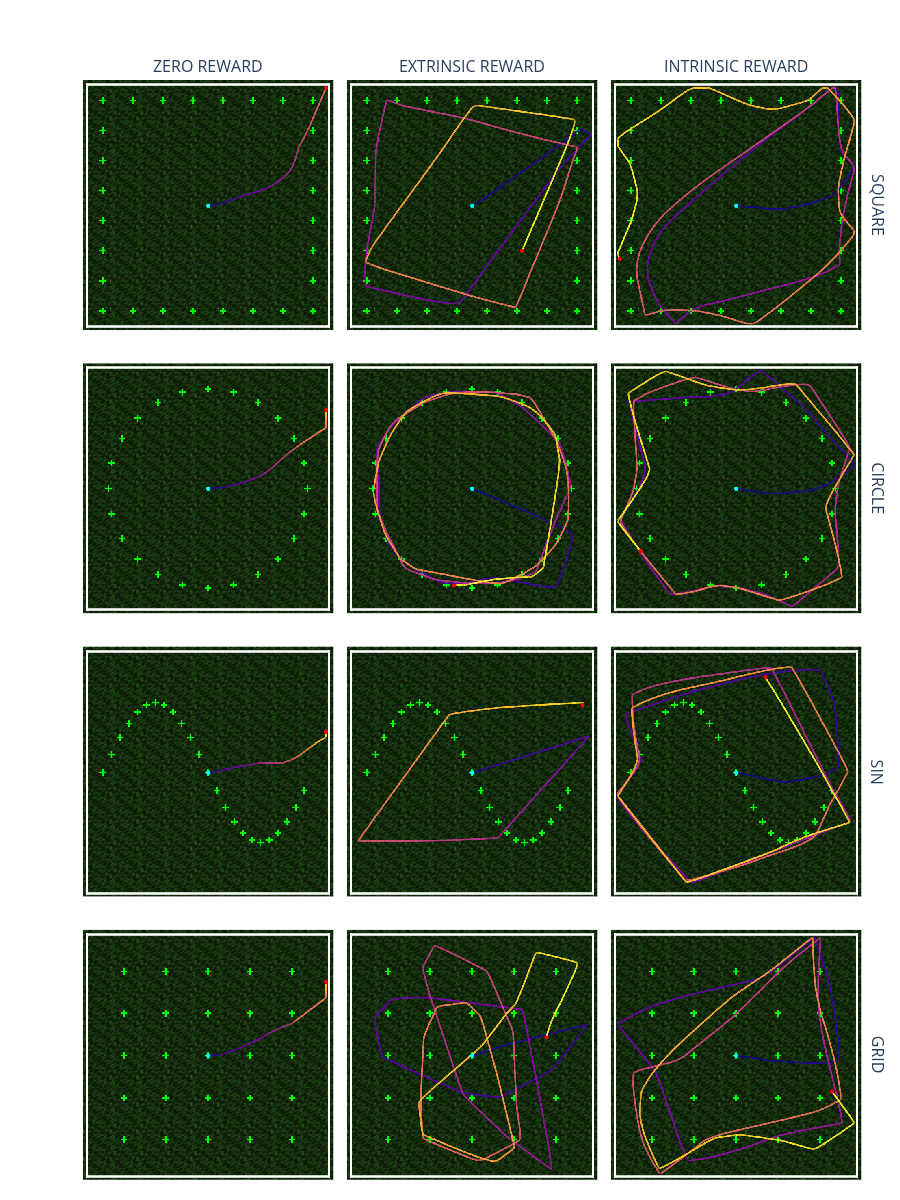
\includegraphics[width=1.0\linewidth]{figuras/trajectory_grid_100.png}
    \caption{Trajetórias produzidas pelas políticas salvas após $9\,533\,440$ passos de treinamento nas distribuições em quadrado, círculo, seno e \textit{grid}, sob as condições sem recompensa, com recompensa extrínseca e com recompensa intrínseca calculada pelo RND, para glaucoma de força $100$.\\
    \textbf{Fonte:} Elaborada pelo autor.}
    \label{fig:trajectories-100}
\end{figure}

Os agentes sem recompensa repetem trajetórias curtas nas quatro distribuições, deslocando-se da posição inicial até uma região próxima à extremidade do ambiente. A semelhança entre esses percursos, apesar da alteração na posição dos recursos, indica que a política não responde à organização dos \textit{medikits}. Esse padrão é coerente com a baixa duração média dos episódios observada durante o treinamento.

Com recompensa extrínseca, os deslocamentos tornam-se extensos. A distribuição circular apresenta a correspondência mais clara entre trajetória e posição dos recursos. Nas distribuições em quadrado e seno, os agentes percorrem grandes polígonos que alcançam diferentes regiões do ambiente, mas não reproduzem precisamente os arranjos. Na distribuição em \textit{grid}, as trajetórias concentram-se principalmente na região central. Apesar dessas diferenças, a elevada duração dos episódios indica que os percursos permitem coletar recursos suficientes para sustentar o agente. A força $100$ compromete a visão mais rapidamente, de modo que a perda de \textit{medikits} próximos do campo visual constitui uma possível explicação para movimentos amplos e menos aderentes às distribuições.

As políticas treinadas com recompensas intrínsecas calculadas pelo RND também produzem trajetórias extensas. Na distribuição circular, os percursos formam um contorno aproximadamente circular. Nas demais distribuições, predominam movimentos amplos próximos às regiões externas do ambiente, com menor correspondência à geometria exata dos recursos. Ainda assim, as trajetórias diferem entre os arranjos e não reproduzem uma única estratégia fixa. Em conjunto com a duração média próxima de $2000$ \textit{ticks}, esse resultado indica que os agentes conseguem encontrar \textit{medikits} mesmo quando a degradação perceptiva dificulta uma navegação diretamente orientada para cada recurso visível.

\subsubsection{Relação entre Recompensa Intrínseca e Precariedade}

A Figura~\ref{fig:intrinsic-reward-100} apresenta a relação entre recompensa intrínseca e precariedade perceptiva para o glaucoma de força $100$. As recompensas foram calculadas pelo módulo RND após $200\,704$ passos de treinamento. A escolha desse checkpoint inicial facilita a observação do mecanismo porque o agente ainda coleta \textit{medikits} com menor frequência. Dessa forma, o episódio apresenta tanto um período suficientemente longo de degradação perceptiva quanto uma coleta posterior, permitindo comparar a recompensa intrínseca antes e depois da restauração da visão. Em checkpoints mais tardios, a maior capacidade de coleta tende a interromper o avanço do glaucoma com maior frequência, tornando menos evidente a relação temporal entre as duas variáveis.

\begin{figure}[h!]
    \centering
    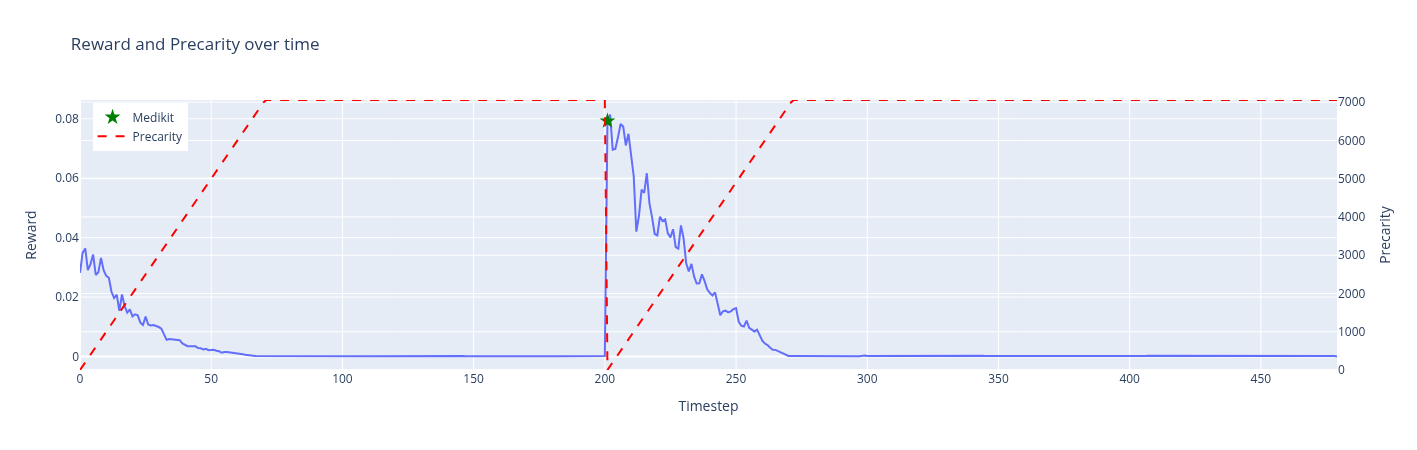
\includegraphics[width=0.9\linewidth]{figuras/intrinsic_reward_100.png}
    \caption{Evolução da recompensa intrínseca calculada pelo módulo RND após $200\,704$ passos de treinamento e da precariedade perceptiva ao longo de um episódio com glaucoma de força $100$. A estrela indica a coleta de um \textit{medikit} e a consequente restauração da visão.\\
    \textbf{Fonte:} Elaborada pelo autor.}
    \label{fig:intrinsic-reward-100}
\end{figure}

No início do episódio, o glaucoma alcança seu nível máximo aproximadamente no instante $70$, mais rapidamente do que na condição de força $50$. Durante esse crescimento, a recompensa intrínseca diminui progressivamente até atingir valores próximos de zero. Enquanto a precariedade permanece máxima, a recompensa também permanece praticamente nula.

Próximo ao instante $200$, a coleta de um \textit{medikit} restaura a visão e produz uma elevação abrupta da recompensa intrínseca, que alcança o maior valor do episódio. Em seguida, conforme a precariedade volta a crescer, a recompensa diminui novamente e retorna a valores próximos de zero por volta do instante $270$. A maior força do glaucoma reduz, portanto, o intervalo durante o qual a observação restaurada permanece pouco degradada e capaz de produzir recompensa elevada.

O padrão observado reforça a relação inversa identificada na força $50$. Estados de elevada precariedade estão associados a recompensas intrínsecas reduzidas, enquanto a restauração da percepção após a coleta de um recurso produz um aumento imediato do erro de predição do RND. Esse resultado constitui mais um indício de que a condição corporal simulada modifica o sinal utilizado pelo aprendizado. A repetição do padrão em diferentes forças de glaucoma fortalece a hipótese de que a precariedade perceptiva está sendo convertida em recompensa.

\subsubsection{Análise Visual com Grad-CAM}

A Figura~\ref{fig:gradcam-100} apresenta mapas de Grad-CAM, método discutido na Seção~\ref{subsubsec:gradcam}, para as três condições de recompensa sob glaucoma de força $100$. A linha superior corresponde às políticas após $100\,352$ passos e a inferior às políticas após $9\,533\,440$ passos. As cores mais quentes indicam regiões com maior contribuição para a saída analisada da política.

\begin{figure}[h!]
    \centering
    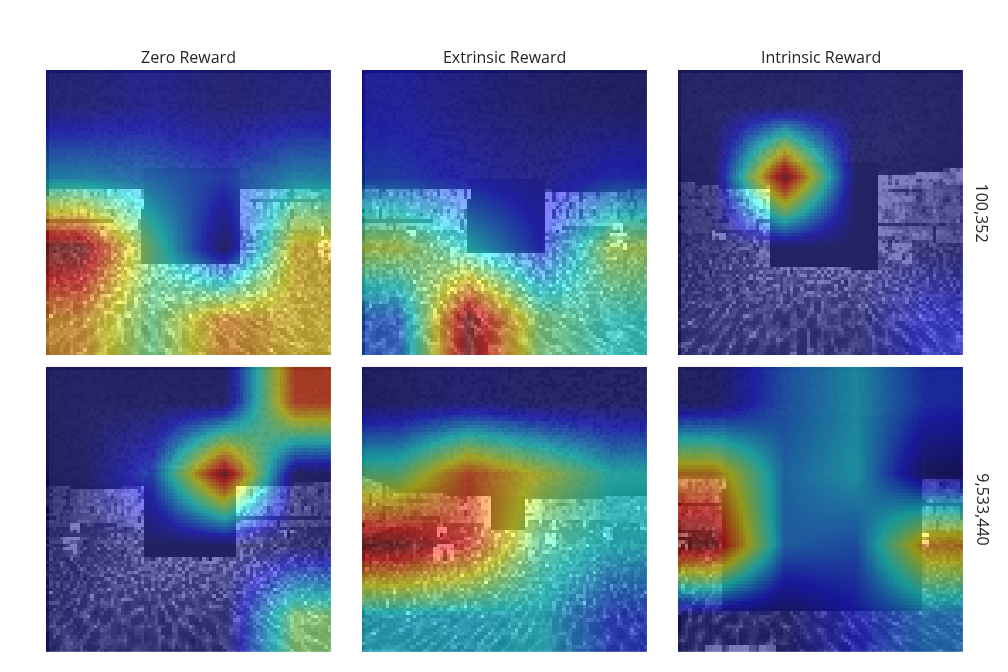
\includegraphics[width=1.0\linewidth]{figuras/gradcam_100.png}
    \caption{Mapas de Grad-CAM para as condições sem recompensa, com recompensa extrínseca e com recompensa intrínseca calculada pelo RND, sob glaucoma de força $100$. A linha superior apresenta as políticas após $100\,352$ passos de treinamento, e a linha inferior apresenta as políticas após $9\,533\,440$ passos. As regiões mais quentes possuem maior relevância para a saída analisada da política segundo o Grad-CAM.\\
    \textbf{Fonte:} Elaborada pelo autor.}
    \label{fig:gradcam-100}
\end{figure}

Na condição sem recompensa, o mapa inicial distribui relevância por grande parte da região inferior, com maior intensidade sobre a parede e o chão à esquerda, enquanto a área central obstruída pelo glaucoma recebe baixa ativação. No estágio final, o foco torna-se mais localizado junto à borda superior da região escurecida e a uma transição entre paredes. A permanência das ativações sobre contrastes, superfícies e limites do glaucoma, sem concentração clara em recursos, é compatível com uma política que não desenvolveu comportamento consistente de coleta.

Na condição com recompensa extrínseca, o mapa inicial destaca principalmente a região inferior central e o chão imediatamente navegável. O \textit{medikit} visível à direita não corresponde ao ponto de maior intensidade. No estágio final, as ativações tornam-se mais amplas e se concentram sobre a parede esquerda, a passagem central e a borda do glaucoma. A região destacada também contém elementos relevantes para a coleta e para a orientação espacial, sugerindo que a política combina informações sobre recursos, superfícies navegáveis e paredes para evitar bloqueios e manter o deslocamento pelo ambiente.

Na condição com recompensa intrínseca, o mapa inicial apresenta um foco intenso e localizado próximo à borda superior esquerda do glaucoma, sem direcionamento evidente para o \textit{medikit} visível na parede direita. Após o treinamento, a relevância se distribui pelas duas laterais da observação, nas quais aparecem partes de \textit{medikits}. A região esquerda, que contém uma porção de um recurso, recebe a maior ativação, enquanto o \textit{medikit} parcialmente visível à direita também é destacado. Esse padrão sugere que a política passou a atribuir relevância aos recursos e aos limites da sala, em vez de responder predominantemente ao contraste produzido pela degradação perceptiva.

Em comparação com a força $50$, os mapas iniciais da força $100$ apresentam influência mais evidente das bordas do glaucoma, coerente com a degradação mais rápida da observação. Nos estágios finais, as condições extrínseca e intrínseca passam a distribuir relevância por elementos do ambiente que podem auxiliar tanto a coleta quanto a navegação, enquanto a condição sem recompensa permanece associada principalmente a características genéricas do cenário e aos limites da obstrução visual.

\subsection{Glaucoma de Força 200}

\subsubsection{Duração Média dos Episódios}

A Figura~\ref{fig:episode-length-200} apresenta a evolução da duração média dos episódios para as três condições de recompensa sob glaucoma de força $200$. As linhas correspondem às médias entre as sementes experimentais, enquanto as regiões sombreadas representam a dispersão de um desvio padrão.

\begin{figure}[h!]
    \centering
    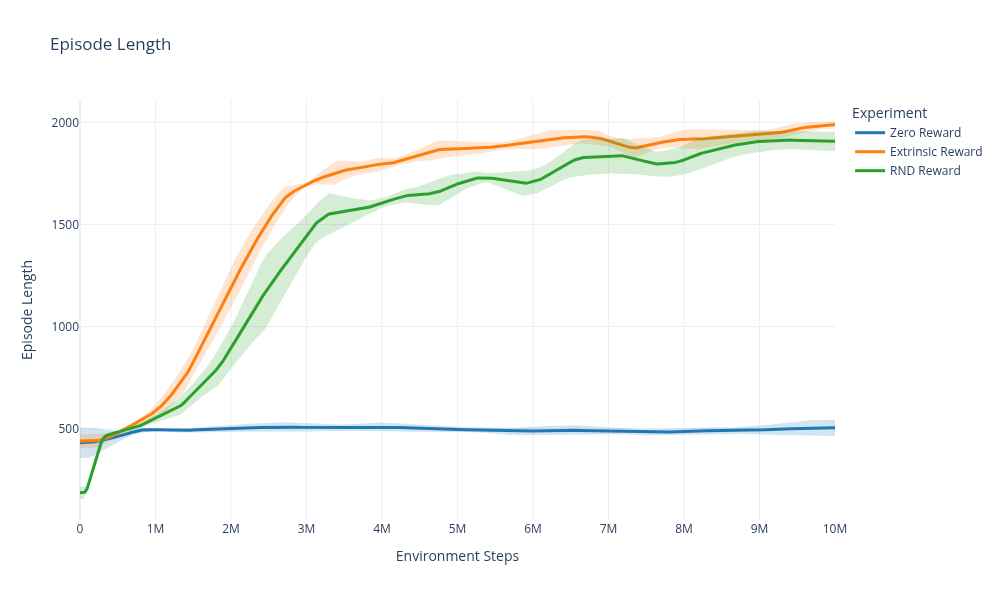
\includegraphics[width=0.9\linewidth]{figuras/episode_length_200.png}
    \caption{Duração média dos episódios ao longo do treinamento nas condições sem recompensa, com recompensa extrínseca e com recompensa intrínseca calculada pelo RND, sob glaucoma de força $200$. As regiões sombreadas representam a variabilidade entre as sementes experimentais.\\
    \textbf{Fonte:} Elaborada pelo autor.}
    \label{fig:episode-length-200}
\end{figure}

Na condição sem recompensa, a duração permanece próxima de $500$ \textit{ticks} ao longo de todo o treinamento. A estabilidade da curva indica que as pequenas variações entre as execuções não correspondem a uma melhoria sistemática da capacidade de sobrevivência. Assim como nas forças anteriores, a ausência de um sinal de reforço impede o desenvolvimento de uma política capaz de coletar recursos de forma consistente.

Com recompensa extrínseca, a duração aumenta rapidamente entre $1$ e $3$ milhões de passos, alcançando aproximadamente $1700$ \textit{ticks}. A partir desse ponto, o crescimento torna-se gradual, e a curva se aproxima de $2000$ \textit{ticks} ao final do treinamento. A faixa de desvio padrão é mais ampla durante a fase inicial de aprendizado e diminui conforme as sementes convergem. Esse resultado mostra que os agentes conseguem aprender a coletar \textit{medikits} e prolongar sua permanência no ambiente mesmo quando a força $200$ produz uma degradação perceptiva muito rápida.

Na condição com recompensa intrínseca calculada pelo RND, o crescimento ocorre mais lentamente. A duração aumenta de maneira acentuada entre aproximadamente $1{,}5$ e $3{,}5$ milhões de passos, quando ultrapassa $1500$ \textit{ticks}. Em seguida, continua crescendo de forma gradual, com oscilações entre $6$ e $8$ milhões de passos, até se aproximar de $1900$ \textit{ticks}. Embora permaneça ligeiramente abaixo da recompensa extrínseca ao final do treinamento, a condição intrínseca apresenta episódios muito mais longos do que a condição sem recompensa. Isso indica que o sinal calculado pelo RND continua sendo suficiente para favorecer uma política de sobrevivência mesmo sob a intensidade mais elevada de glaucoma analisada.

\subsubsection{Análise das Trajetórias}

A Figura~\ref{fig:trajectories-200} apresenta as trajetórias produzidas nas quatro distribuições de \textit{medikits}. Os episódios de avaliação foram executados com as políticas salvas após $9\,533\,440$ passos de treinamento. Esse checkpoint corresponde a um estágio próximo do limite de $10$ milhões de passos e posterior à fase principal de crescimento das curvas de duração dos episódios. Assim, a análise se concentra no comportamento desenvolvido em uma etapa avançada do aprendizado, quando as políticas já haviam sido expostas a uma quantidade ampla de experiências sob a degradação perceptiva mais intensa.

\begin{figure}[h!]
    \centering
    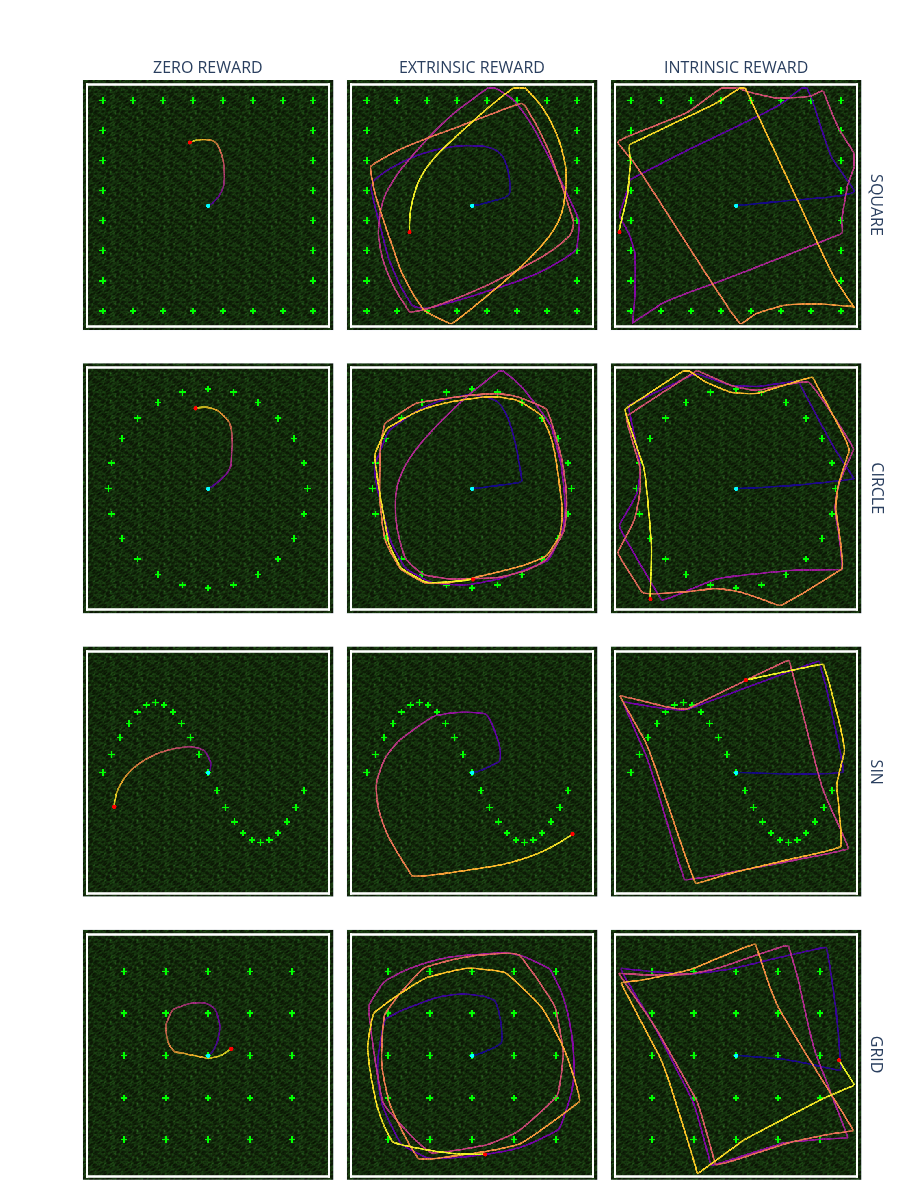
\includegraphics[width=1.0\linewidth]{figuras/trajectory_grid_200.png}
    \caption{Trajetórias produzidas pelas políticas salvas após $9\,533\,440$ passos de treinamento nas distribuições em quadrado, círculo, seno e \textit{grid}, sob as condições sem recompensa, com recompensa extrínseca e com recompensa intrínseca calculada pelo RND, para glaucoma de força $200$.\\
    \textbf{Fonte:} Elaborada pelo autor.}
    \label{fig:trajectories-200}
\end{figure}

Os agentes sem recompensa realizam percursos curtos e pouco relacionados à disposição dos recursos. Nas distribuições em quadrado, círculo e seno, as trajetórias se limitam a pequenos arcos iniciados no centro do ambiente. Na distribuição em \textit{grid}, observa-se um movimento circular igualmente restrito. A alteração do percurso não acompanha as diferentes organizações dos \textit{medikits} e não produz coleta suficiente para aumentar a duração dos episódios.

Com recompensa extrínseca, os agentes percorrem regiões amplas do ambiente. A distribuição circular apresenta novamente a maior correspondência entre as trajetórias e a posição dos recursos. Nas distribuições em quadrado e \textit{grid}, os percursos formam contornos extensos que interceptam diferentes \textit{medikits}, embora não reproduzam exatamente os arranjos. Na distribuição em seno, as trajetórias alcançam parte da curva formada pelos recursos, mas também atravessam regiões externas. A elevada duração média dos episódios indica que esses deslocamentos permitem coletar recursos suficientes, apesar da baixa aderência à geometria de algumas distribuições.

As políticas treinadas com recompensas intrínsecas calculadas pelo RND também produzem trajetórias extensas, mas predominantemente poligonais e próximas aos limites do ambiente. Na distribuição circular, os percursos contornam grande parte dos recursos, ainda que de maneira menos regular do que na condição extrínseca. Nas demais distribuições, a correspondência com a disposição dos \textit{medikits} é limitada. Ainda assim, as diferenças entre os percursos e a duração média próxima de $1900$ \textit{ticks} mostram que os agentes conseguem interceptar recursos e manter-se no ambiente. Uma possível explicação para a menor precisão espacial é que, sob glaucoma de força $200$, os \textit{medikits} deixam rapidamente de ser visíveis, favorecendo estratégias de deslocamento amplo que aumentam a probabilidade de encontrá-los durante o percurso.

\subsubsection{Relação entre Recompensa Intrínseca e Precariedade}

A Figura~\ref{fig:intrinsic-reward-200} apresenta a evolução conjunta da recompensa intrínseca e da precariedade perceptiva sob glaucoma de força $200$. As recompensas foram calculadas pelo módulo RND após $200\,704$ passos de treinamento. Esse estágio inicial foi utilizado para que o episódio incluísse períodos prolongados sem coleta, nos quais a degradação perceptiva pudesse alcançar seu nível máximo, e um evento posterior de coleta que permitisse observar a restauração da visão. Como o agente ainda não havia aprendido a encontrar recursos com elevada frequência, o contraste entre os estados anteriores e posteriores à coleta torna-se mais claro. Em políticas mais avançadas, a sucessão de coletas reduziria a duração desses intervalos e dificultaria a análise isolada do efeito de cada \textit{medikit}.

\begin{figure}[h!]
    \centering
    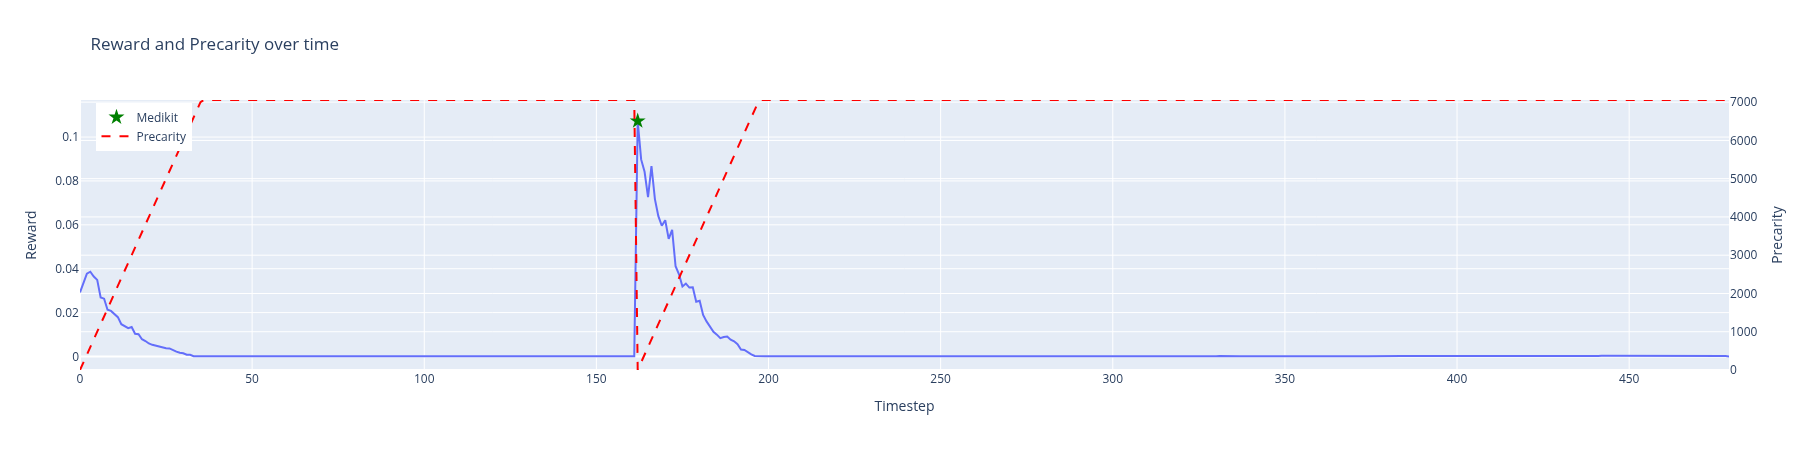
\includegraphics[width=0.9\linewidth]{figuras/intrinsic_reward_200.png}
    \caption{Evolução da recompensa intrínseca calculada pelo módulo RND após $200\,704$ passos de treinamento e da precariedade perceptiva ao longo de um episódio com glaucoma de força $200$. A estrela indica a coleta de um \textit{medikit} e a consequente restauração da visão.\\
    \textbf{Fonte:} Elaborada pelo autor.}
    \label{fig:intrinsic-reward-200}
\end{figure}

No início do episódio, a precariedade alcança seu nível máximo aproximadamente no instante $35$. Durante esse intervalo, a recompensa intrínseca apresenta uma elevação inicial e, em seguida, diminui até atingir valores próximos de zero. A recompensa permanece praticamente nula enquanto a visão está totalmente degradada, indicando que essas observações produzem pouco erro de predição para o RND.

Próximo ao instante $162$, a coleta de um \textit{medikit} restaura a visão e produz o maior pico de recompensa intrínseca do episódio. Após a restauração, a precariedade volta a crescer rapidamente e alcança novamente o nível máximo por volta do instante $198$. No mesmo intervalo, a recompensa diminui progressivamente até retornar a valores próximos de zero. Em comparação com as forças $50$ e $100$, o período durante o qual a observação permanece pouco degradada é ainda menor.

O resultado mantém o padrão observado nas demais intensidades de glaucoma. A restauração da visão está associada a um aumento abrupto da recompensa intrínseca, enquanto a degradação perceptiva reduz esse sinal. Na força $200$, porém, a rápida perda de visão limita temporalmente a oportunidade de obter recompensas elevadas após a coleta. A reprodução dessa relação inversa na intensidade mais extrema analisada reforça o indício de que a precariedade perceptiva modifica sistematicamente a recompensa calculada pelo RND.

\subsubsection{Análise Visual com Grad-CAM}

A Figura~\ref{fig:gradcam-200} apresenta mapas de Grad-CAM, método discutido na Seção~\ref{subsubsec:gradcam}, para as três condições de recompensa sob glaucoma de força $200$. A linha superior corresponde às políticas após $100\,352$ passos e a inferior às políticas após $9\,533\,440$ passos. As cores mais quentes indicam regiões com maior contribuição para a saída analisada da política.

\begin{figure}[h!]
    \centering
    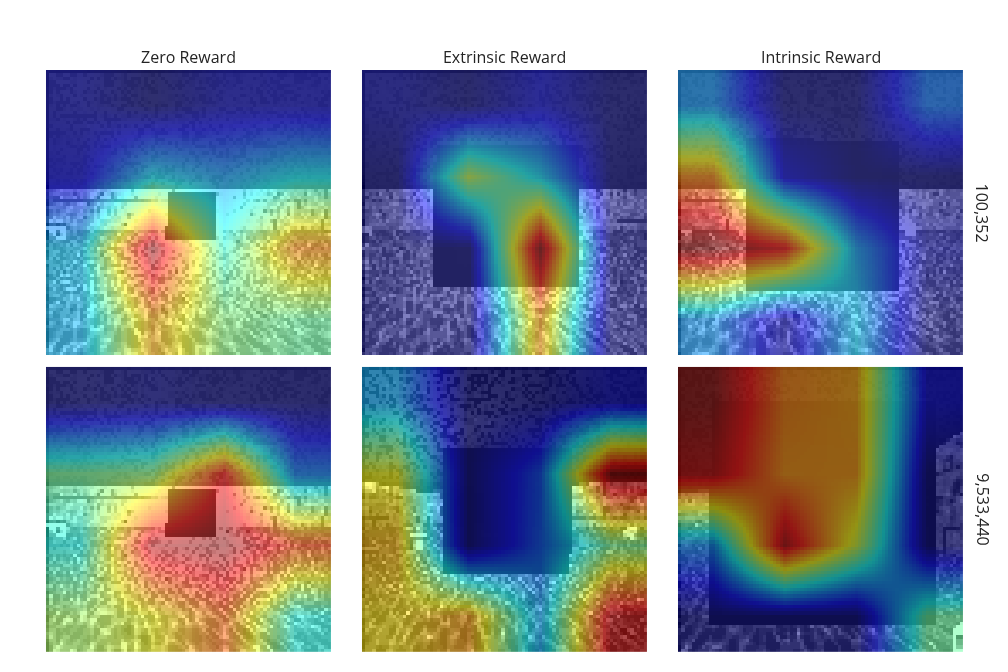
\includegraphics[width=1.0\linewidth]{figuras/gradcam_200.png}
    \caption{Mapas de Grad-CAM para as condições sem recompensa, com recompensa extrínseca e com recompensa intrínseca calculada pelo RND, sob glaucoma de força $200$. A linha superior apresenta as políticas após $100\,352$ passos de treinamento, e a linha inferior apresenta as políticas após $9\,533\,440$ passos. As regiões mais quentes possuem maior relevância para a saída analisada da política segundo o Grad-CAM.\\
    \textbf{Fonte:} Elaborada pelo autor.}
    \label{fig:gradcam-200}
\end{figure}

Na condição sem recompensa, os mapas inicial e final distribuem relevância por regiões amplas do chão, das paredes e das bordas do glaucoma. No estágio final, a maior ativação permanece próxima à área escurecida e às transições entre superfícies, sem concentração clara sobre recursos. Esse padrão é compatível com uma política que responde a características genéricas do cenário e não desenvolve uma estratégia consistente de coleta.

Na condição com recompensa extrínseca, o mapa inicial destaca a passagem central e a borda inferior da região obstruída. Após o treinamento, a ativação se distribui principalmente pela parede direita, pelo chão e pela parte superior da observação, enquanto o \textit{medikit} parcialmente visível não constitui isoladamente o principal foco. Esse padrão sugere que a política atribui maior relevância a referências que auxiliam na navegação, como paredes, limites entre superfícies e a região do céu, do que diretamente aos recursos. Sob glaucoma de força $200$, orientar-se enquanto a visão ainda está disponível é especialmente importante, pois a degradação rápida pode impedir a identificação posterior dos \textit{medikits}. A utilização da geometria do ambiente pode, portanto, ajudar o agente a manter uma direção de deslocamento e alcançar regiões nas quais os recursos provavelmente serão encontrados.

Na condição com recompensa intrínseca, o mapa inicial concentra-se na lateral esquerda e na borda do glaucoma. No estágio final, a ativação torna-se extensa e abrange a parte superior da observação, as paredes e os limites da região degradada, enquanto o recurso parcialmente visível à direita recebe menor relevância. Assim como na condição extrínseca, o foco parece estar menos nos \textit{medikits} individualmente e mais nas referências espaciais que permitem ao agente orientar seu movimento antes que a visão seja amplamente comprometida. A estrutura do céu, das paredes e das passagens pode fornecer uma direção geral para alcançar novas regiões do ambiente, aumentando a possibilidade de interceptar recursos mesmo quando eles deixam de ser diretamente visíveis. Esse comportamento é compatível com trajetórias amplas e pouco aderentes às distribuições, mas ainda capazes de prolongar a sobrevivência.

Em comparação com as forças $50$ e $100$, a força $200$ produz mapas mais dominados por regiões amplas, pela área escurecida e por referências estruturais do cenário. Tanto na condição extrínseca quanto na intrínseca, céu, paredes, chão e passagens parecem exercer maior influência do que os \textit{medikits} isoladamente. Essa diferença indica que a perda rapidamente iminente da visão altera a estratégia visual da política. Em vez de depender apenas da identificação precisa dos recursos, o agente utiliza a geometria disponível para se orientar em direção a regiões onde poderá encontrá-los. Dessa forma, a navegação baseada na estrutura geral do ambiente pode compensar parcialmente a curta janela durante a qual os \textit{medikits} permanecem visíveis.

\subsection{Glaucoma de Força 0}

A condição de força $0$ é analisada por último por constituir uma ablação do mecanismo proposto. Nessa configuração, o agente mantém a visão inalterada durante todo o episódio, de modo que a ausência de coleta de \textit{medikits} não produz degradação perceptiva e a coleta não restaura qualquer capacidade visual. O RND continua calculando recompensas intrínsecas a partir das observações, mas essas recompensas deixam de estar acopladas à manutenção da condição perceptiva do agente. Essa condição permite avaliar se a curiosidade, isoladamente, é suficiente para produzir uma política de sobrevivência ou se a precariedade é necessária para relacionar a coleta de recursos à continuidade da obtenção de recompensa intrínseca.

\subsubsection{Duração Média dos Episódios}

A Figura~\ref{fig:episode-length-0} apresenta a evolução da duração média dos episódios na ausência de glaucoma. As linhas representam as médias entre as sementes experimentais e as regiões sombreadas correspondem à dispersão de um desvio padrão.

\begin{figure}[h!]
    \centering
    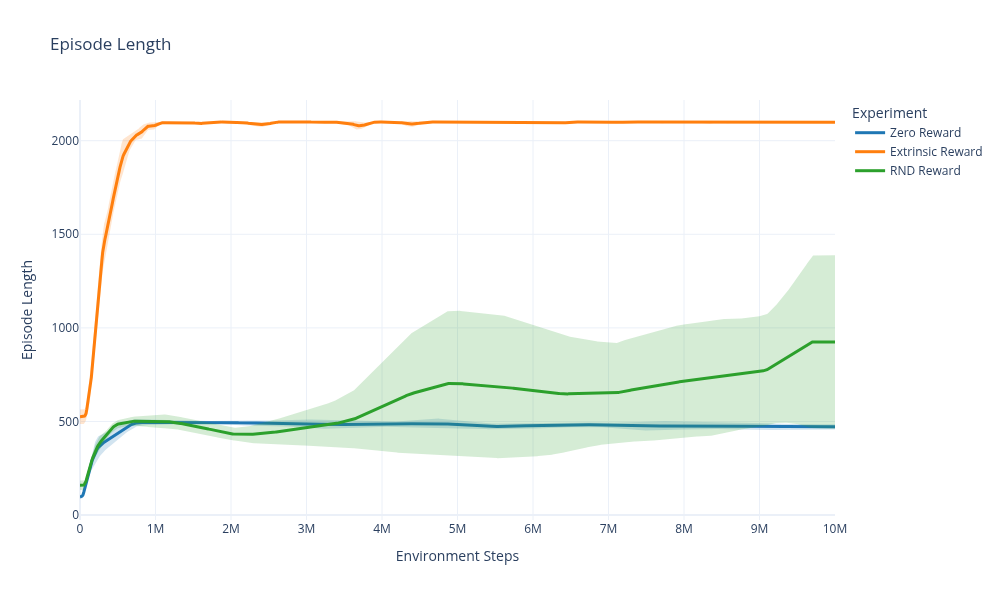
\includegraphics[width=0.9\linewidth]{figuras/episode_length_0.png}
    \caption{Duração média dos episódios ao longo do treinamento nas condições sem recompensa, com recompensa extrínseca e com recompensa intrínseca calculada pelo RND, sob glaucoma de força $0$. As regiões sombreadas representam a variabilidade entre as sementes experimentais.\\
    \textbf{Fonte:} Elaborada pelo autor.}
    \label{fig:episode-length-0}
\end{figure}

Na condição sem recompensa, a duração aumenta apenas no início do treinamento e se estabiliza próxima de $480$ \textit{ticks}. Esse comportamento é semelhante ao observado nas demais forças e confirma que o PPO não desenvolve uma política de sobrevivência quando não recebe um sinal capaz de distinguir ações ou estados relevantes para a tarefa.

Com recompensa extrínseca, a duração cresce rapidamente e alcança o limite de $2100$ \textit{ticks} antes de $1$ milhão de passos. A curva permanece estável nesse nível durante praticamente todo o restante do treinamento, com baixa variabilidade entre as sementes. Esse é o aprendizado mais rápido entre as forças analisadas, o que é compatível com a ausência de degradação visual. Como o agente mantém acesso integral às observações e recebe recompensa direta pela coleta, pode localizar os \textit{medikits} e aprender a utilizá-los sem enfrentar a perda progressiva de informação perceptiva presente nas demais condições.

O comportamento da condição com recompensa intrínseca é substancialmente diferente. A duração inicialmente se aproxima de $500$ \textit{ticks}, mas não apresenta a transição consistente para episódios próximos do limite máximo observada nas forças $50$, $100$ e $200$. A média cresce lentamente após aproximadamente $3{,}5$ milhões de passos e alcança cerca de $900$ \textit{ticks} ao final do treinamento. Entretanto, esse aumento é acompanhado por uma faixa de desvio padrão muito ampla, especialmente após $4$ milhões de passos. A elevada dispersão indica que o resultado não é reproduzido de forma consistente entre as sementes e que parte das execuções permanece próxima ao desempenho da condição sem recompensa.

Portanto, o crescimento da média não deve ser interpretado como evidência de uma política robusta de sobrevivência. Sem glaucoma, o RND ainda incentiva a exploração de observações novas, e essa exploração pode levar algumas execuções a encontrar \textit{medikits} incidentalmente ou a desenvolver padrões de movimento que prolonguem parcialmente os episódios. Contudo, não existe um mecanismo que atribua valor específico à manutenção da visão, pois ela nunca é perdida. A diferença em relação às forças positivas de glaucoma está tanto no desempenho final quanto na reprodutibilidade. Com precariedade perceptiva, as sementes convergem para episódios longos. Sem precariedade, o ganho é limitado e altamente dependente da semente.

\subsubsection{Análise das Trajetórias}

A Figura~\ref{fig:trajectories-0} apresenta as trajetórias produzidas nas quatro distribuições de \textit{medikits}. Os episódios de avaliação foram executados com as políticas salvas após $9\,132\,032$ passos de treinamento. Esse checkpoint representa uma política em estágio avançado e próximo do orçamento total de treinamento. Sua utilização permite verificar se, mesmo após milhões de interações, a ausência de precariedade ainda impede a emergência de uma estratégia consistente na condição com recompensa intrínseca. O ponto analisado não pressupõe que todas as condições tenham convergido, mas permite examinar o comportamento adquirido em uma etapa tardia do treinamento.

\begin{figure}[h!]
    \centering
    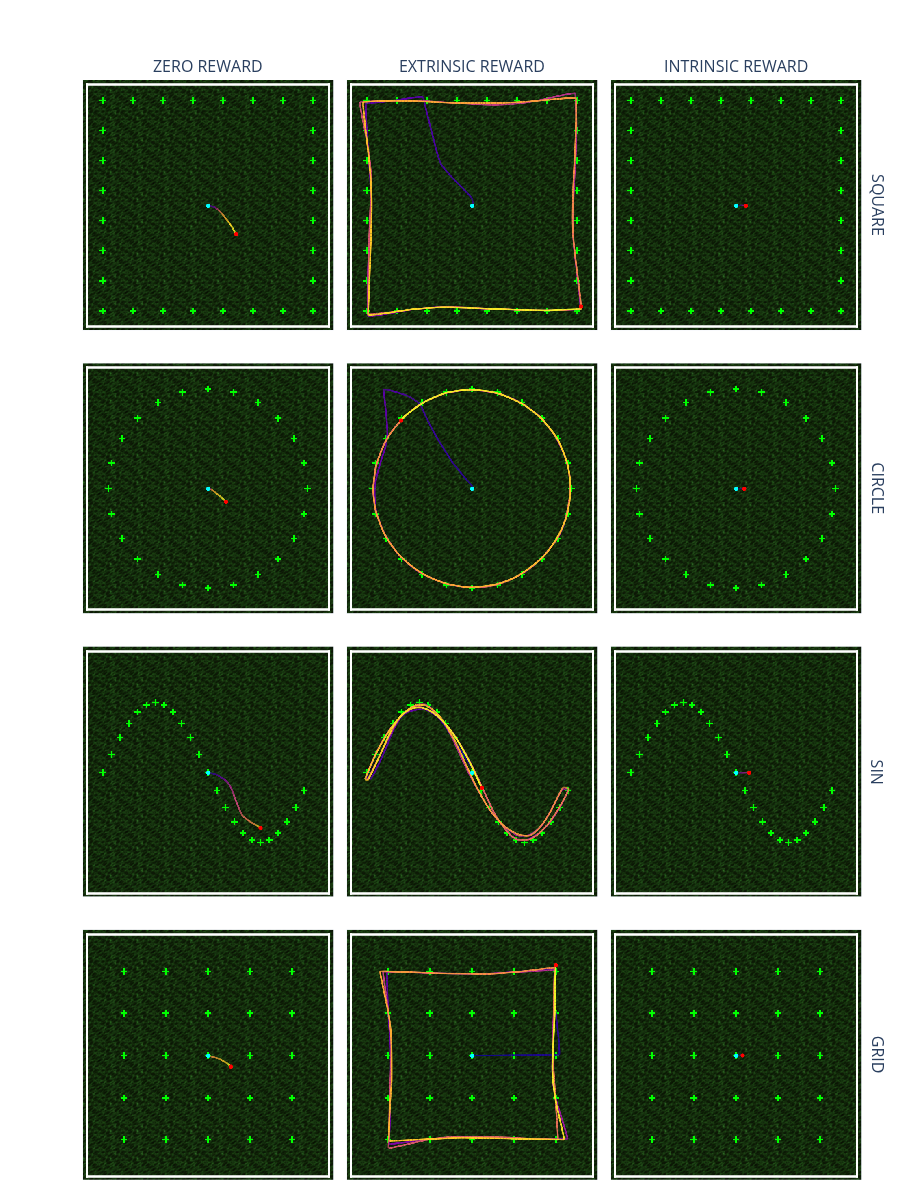
\includegraphics[width=1.0\linewidth]{figuras/trajectory_grid_0.png}
    \caption{Trajetórias produzidas pelas políticas salvas após $9\,132\,032$ passos de treinamento nas distribuições em quadrado, círculo, seno e \textit{grid}, sob as condições sem recompensa, com recompensa extrínseca e com recompensa intrínseca calculada pelo RND, para glaucoma de força $0$.\\
    \textbf{Fonte:} Elaborada pelo autor.}
    \label{fig:trajectories-0}
\end{figure}

Os agentes treinados sem recompensa realizam deslocamentos muito curtos a partir da posição inicial. As trajetórias são semelhantes nas quatro distribuições e terminam antes de alcançar a maior parte dos recursos. Esse resultado é coerente com a duração média próxima de $480$ \textit{ticks} e não apresenta evidências de que a política utilize a disposição dos \textit{medikits} para orientar suas ações.

A condição com recompensa extrínseca apresenta um contraste claro. Na distribuição em quadrado, as trajetórias acompanham os quatro lados formados pelos recursos. Na distribuição circular, os agentes percorrem o contorno do círculo. Na distribuição em seno, os caminhos reproduzem a curva com elevada proximidade. Na distribuição em \textit{grid}, as trajetórias percorrem principalmente o perímetro do arranjo, interceptando sucessivos \textit{medikits}. A correspondência entre os caminhos e as diferentes geometrias mostra que a arquitetura e o algoritmo são capazes de aprender políticas sensíveis à organização espacial dos recursos quando o sinal de recompensa fornece diretamente essa orientação. Esse resultado também afasta a possibilidade de que o baixo desempenho da condição intrínseca seja explicado apenas por limitações do ambiente, do espaço de ações ou da rede utilizada.

Nas políticas treinadas com recompensas intrínsecas calculadas pelo RND, os agentes permanecem praticamente imóveis nas quatro distribuições. Os pequenos deslocamentos próximos à posição inicial não acompanham os recursos e são insuficientes para caracterizar uma estratégia de busca. Além disso, a semelhança das trajetórias diante de arranjos distintos indica que a política avaliada não utiliza a organização espacial dos \textit{medikits} para orientar seu comportamento. Esse resultado ajuda a interpretar a elevada variabilidade observada no gráfico de duração. Ainda que algumas sementes possam alcançar episódios mais longos, a política representada na análise comportamental não desenvolve uma estratégia consistente de coleta.

A comparação com as forças positivas de glaucoma é central para a hipótese do trabalho. Quando há degradação perceptiva, deixar de coletar recursos compromete progressivamente as observações e reduz a recompensa intrínseca disponível. A coleta restaura a visão e cria uma consequência relevante para o mecanismo de curiosidade. Na força $0$, a percepção permanece preservada independentemente das ações do agente. Assim, coletar ou ignorar um \textit{medikit} não altera sua capacidade futura de perceber novidades. O recurso deixa de participar da dinâmica da recompensa intrínseca, e a curiosidade não se converte de maneira confiável em comportamento de manutenção da viabilidade.

\subsubsection{Relação entre Recompensa Intrínseca e Precariedade}

A Figura~\ref{fig:intrinsic-reward-0} apresenta a recompensa intrínseca calculada pelo módulo RND após $301\,056$ passos de treinamento. Esse checkpoint inicial foi utilizado porque o agente ainda não coletava \textit{medikits} com frequência, permitindo observar um intervalo prolongado sem coleta e um evento posterior de obtenção do recurso. Essa configuração facilita verificar se a coleta, por si só, produz alguma alteração sistemática na recompensa intrínseca. Diferentemente das forças positivas, entretanto, a ausência de coleta não causa degradação visual e a obtenção do recurso não restaura a percepção. Como a força do glaucoma é igual a $0$, a precariedade permanece nula durante todo o episódio.

\begin{figure}[h!]
    \centering
    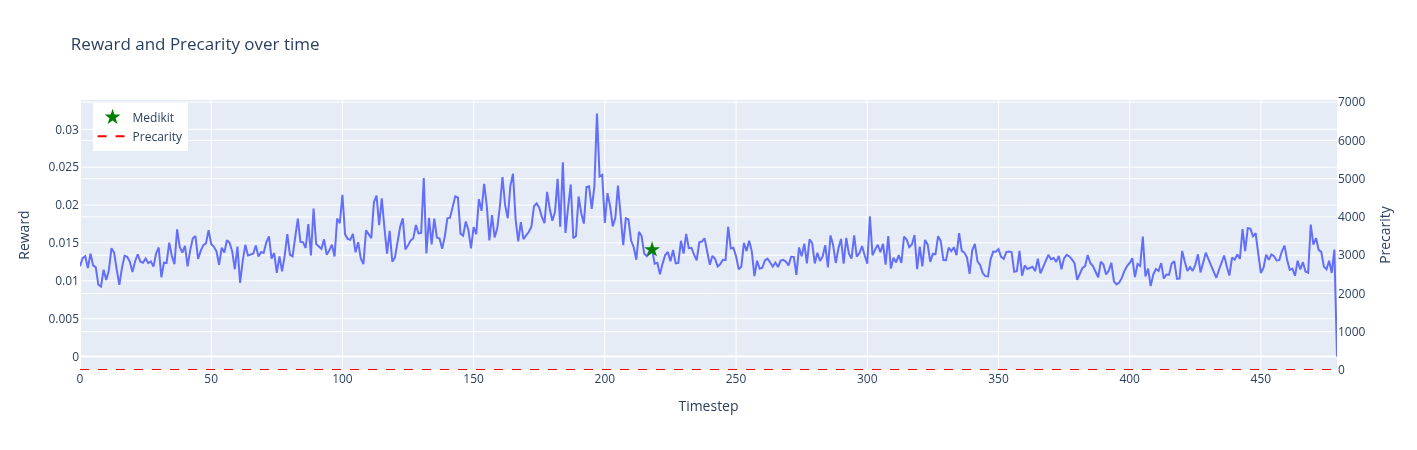
\includegraphics[width=0.9\linewidth]{figuras/intrinsic_reward_0.png}
    \caption{Evolução da recompensa intrínseca calculada pelo módulo RND após $301\,056$ passos de treinamento e da precariedade perceptiva ao longo de um episódio com glaucoma de força $0$. A estrela indica a coleta de um \textit{medikit}.\\
    \textbf{Fonte:} Elaborada pelo autor.}
    \label{fig:intrinsic-reward-0}
\end{figure}

Ao contrário das condições com forças $50$, $100$ e $200$, a linha de precariedade permanece constante no valor mínimo. A recompensa intrínseca continua apresentando oscilações porque o RND responde à novidade das observações produzidas durante a interação. Entretanto, essas variações não acompanham qualquer alteração da condição perceptiva, uma vez que a visão não se degrada nem é restaurada.

A coleta de um \textit{medikit}, indicada aproximadamente no instante $218$, não é seguida por um pico abrupto de recompensa. Os valores posteriores permanecem na mesma faixa de variação observada antes da coleta e chegam a diminuir imediatamente após o evento. Isso contrasta com as forças positivas de glaucoma, nas quais a coleta restaura a visão e produz uma elevação clara do erro de predição. Na força $0$, o \textit{medikit} recupera a vida do agente, mas não transforma a observação visual por meio do mecanismo proposto. Consequentemente, o RND não recebe um sinal perceptivo que diferencie sistematicamente o instante posterior à coleta.

Esse resultado esclarece que a simples existência de recompensa intrínseca não é suficiente para orientar o agente à manutenção de sua viabilidade. O RND continua produzindo valores diferentes de zero, mas tais valores refletem novidades visuais gerais e não a necessidade de coletar recursos. Sem precariedade, não há perda de uma condição que precise ser restaurada e, portanto, não se estabelece a relação funcional entre manutenção corporal, percepção e curiosidade pretendida neste trabalho.

\subsubsection{Análise Visual com Grad-CAM}

A Figura~\ref{fig:gradcam-0} apresenta mapas de Grad-CAM, método discutido na Seção~\ref{subsubsec:gradcam}, para as três condições de recompensa sob glaucoma de força $0$. A linha superior corresponde às políticas após $100\,352$ passos e a inferior às políticas após $9\,132\,032$ passos. As cores mais quentes indicam regiões com maior contribuição para a saída analisada da política.

\begin{figure}[h!]
    \centering
    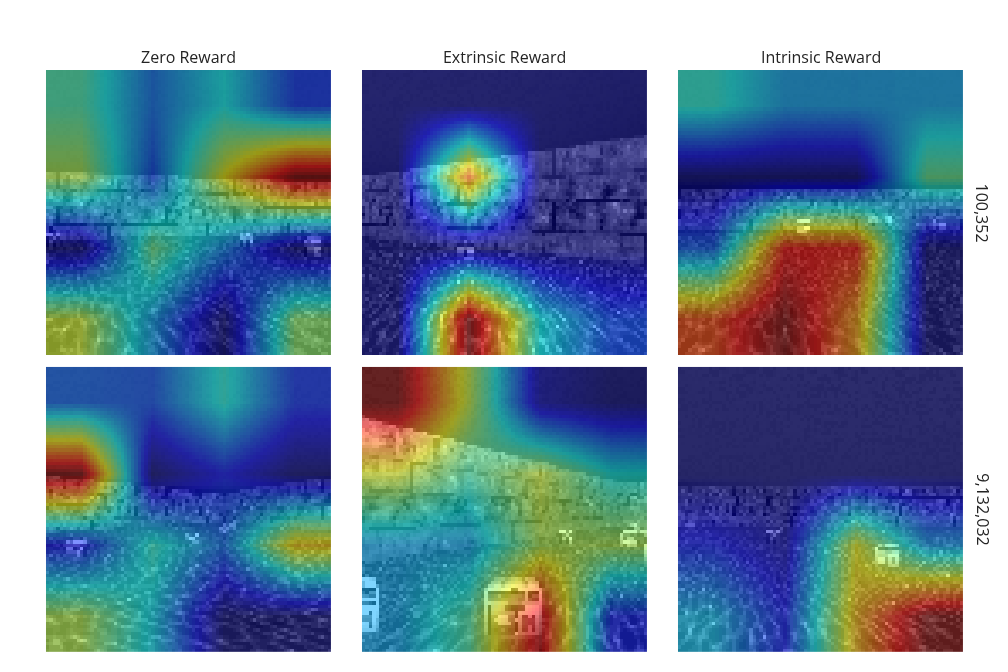
\includegraphics[width=1.0\linewidth]{figuras/gradcam_0.png}
    \caption{Mapas de Grad-CAM para as condições sem recompensa, com recompensa extrínseca e com recompensa intrínseca calculada pelo RND, sob glaucoma de força $0$. A linha superior apresenta as políticas após $100\,352$ passos de treinamento, e a linha inferior apresenta as políticas após $9\,132\,032$ passos. As regiões mais quentes possuem maior relevância para a saída analisada da política segundo o Grad-CAM.\\
    \textbf{Fonte:} Elaborada pelo autor.}
    \label{fig:gradcam-0}
\end{figure}

Na condição sem recompensa, os mapas distribuem relevância por regiões amplas do cenário. No estágio inicial, as maiores ativações aparecem próximas à parede direita e às transições entre céu, paredes e chão. No estágio final, os focos permanecem associados às laterais e ao piso, sem concentração consistente sobre os \textit{medikits} visíveis. Esse padrão é compatível com uma política guiada por características genéricas do ambiente e sem uma estratégia de coleta.

Na condição com recompensa extrínseca, o mapa inicial apresenta focos localizados sobre os \textit{medikits} visíveis nas regiões central superior e inferior. Após o treinamento, o recurso próximo à parte inferior continua recebendo a maior ativação, enquanto outros itens presentes na observação também recebem relevância. Como não há degradação perceptiva, os recursos permanecem visíveis e podem ser utilizados diretamente para orientar as ações. Esse resultado é coerente com as trajetórias que acompanham as distribuições e com a rápida convergência para episódios de duração máxima.

Na condição com recompensa intrínseca, o mapa inicial é amplo e concentra-se principalmente no chão e nas paredes, sem um foco preciso sobre recursos. No estágio final, um \textit{medikit} visível à direita recebe alguma relevância, mas a maior ativação permanece distribuída pela região inferior e pelas transições entre superfícies. Assim, embora a política seja capaz de utilizar partes da observação que contêm recursos, os mapas não indicam uma priorização visual tão clara quanto na condição extrínseca. Esse comportamento é compatível com as trajetórias curtas e com a ausência de aprendizado robusto de coleta.

A comparação é especialmente relevante porque, na força $0$, nenhuma parte da observação é ocultada pelo glaucoma. A condição extrínseca demonstra que a arquitetura e o Grad-CAM conseguem produzir focos claros sobre os \textit{medikits} quando esses itens estão diretamente associados à recompensa. Na condição intrínseca, porém, a manutenção da visão independe da coleta e os recursos não provocam uma transformação perceptiva relevante para o RND. A ausência de um foco consistente nos \textit{medikits} reforça, portanto, que a curiosidade isolada não estabelece o mesmo vínculo entre percepção, coleta e sobrevivência observado nas condições com precariedade.

\section{Síntese Comparativa dos Resultados}

A comparação entre as forças $0$, $50$, $100$ e $200$ mostra que a variável de vida, isoladamente, não orienta o aprendizado. Seu valor apenas determina o encerramento do episódio e não é fornecido à política nem utilizado no cálculo da recompensa. Na condição sem recompensa, os agentes permanecem próximos de $500$ \textit{ticks} em todas as forças, o que indica que a possibilidade de morte não é suficiente para produzir uma política de manutenção. Com recompensa extrínseca, todas as forças alcançam durações próximas do limite de $2100$ \textit{ticks}, pois a permanência no ambiente e a coleta são diretamente valorizadas. A recompensa resolve a tarefa, mas também informa previamente a solução esperada.

A comparação mais importante ocorre entre as configurações intrínsecas. O PPO, a arquitetura, o RND e a definição da recompensa permanecem inalterados, enquanto apenas a força do glaucoma modifica a velocidade de deterioração do corpo perceptivo. Mesmo assim, as forças $50$, $100$ e $200$ convergem para episódios próximos de $1900$ a $2000$ \textit{ticks}, enquanto a força $0$ apresenta menor desempenho e elevada variabilidade entre as sementes. As diferenças comportamentais não foram produzidas por uma nova regra de aprendizado nem por uma recompensa específica para cada força. Elas surgiram da alteração do corpo artificial e da forma como ele passou a se relacionar com o ambiente.

Esse contraste mostra como a curiosidade pode ser modulada por meio do corpo. Na força $0$, coletar ou ignorar um \textit{medikit} não modifica a percepção e, portanto, não altera de maneira sistemática a recompensa produzida pelo RND. Nas forças positivas, permanecer sem coletar degrada a visão, torna as observações mais pobres e reduz a recompensa intrínseca. A coleta restaura a percepção e produz um aumento do erro de predição. Desse modo, o \textit{medikit} deixa de ser apenas um objeto presente no cenário e adquire significado funcional por recuperar uma condição necessária à continuidade da exploração.

As trajetórias e os mapas de Grad-CAM reforçam que corpos perceptivos diferentes favorecem comportamentos distintos. Com o aumento da força do glaucoma, as políticas passam de uma navegação mais orientada pela posição visível dos recursos para estratégias mais amplas, apoiadas também em paredes, chão, céu e limites da obstrução. Esse resultado é consistente com a perspectiva apresentada por \citeauthoronline{yuri-ambiente-rico} (\citeyear{yuri-ambiente-rico}; \citeyear{yuri-sem-objetivo}), segundo a qual alterações no corpo, na percepção e no ambiente modificam as regularidades disponíveis ao agente e os comportamentos que podem emergir.

Se o único objetivo fosse resolver a tarefa, a recompensa extrínseca seria uma solução mais direta. A contribuição da proposta está em mostrar que um mecanismo geral de curiosidade pode ser orientado pela construção do corpo e do ambiente, sem alterar o algoritmo de aprendizado ou introduzir recompensas específicas para os comportamentos desejados nas diferentes forças. Em vez de informar ao agente que deve coletar recursos, o experimento cria condições nas quais a coleta modifica sua própria capacidade de continuar percebendo e obtendo novidade.

Essa dinâmica oferece uma aproximação limitada à ideia de autoconstrução. O agente não produz seus componentes, não define seus limites de viabilidade e não realiza autopoiese. Contudo, precisa agir para recuperar uma capacidade corporal que se deteriora ao longo do tempo. Nas configurações avaliadas, essa exigência de reconstrução funcional foi suficiente para favorecer políticas de sobrevivência e constitui um pequeno passo experimental na direção de agentes cujo comportamento dependa das consequências de suas ações sobre sua própria condição.
